\documentclass[11pt, a4paper]{article}
\usepackage[utf8]{inputenc}
\usepackage{amsmath, amssymb}
\usepackage{graphicx}
\usepackage{hyperref}
\usepackage{geometry}
\geometry{margin=1in}

\title{EE 325 Digital Signal Processing \\ Laboratory Assignment 1: Frequency Estimation}
\author{PERERA J.D.T. \\ E/21/291}
\date{\today}

\begin{document}
\maketitle

\section{Aim and Objectives}
\textbf{Aim:} To determine the frequency of a sinusoidal using various signal processing techniques.

\textbf{Objectives:} To determine the spectral content of a sampled signal using:
\begin{enumerate}
    \item The discrete Fourier transform (DFT)
    \item The spectrogram (STFT)
    \item The autocorrelation function
    \item The Periodogram
    \item The Pisarenko harmonic decomposition / MUSIC
    \item The Auto-regressive (AR) model
\end{enumerate}

\section{Task 1: Signal Construction}
Based on the E-number E/21/291, $a=2, b=9, c=1$.
Frequencies are assigned as:
$$ f_1 = 10 + 2 = 12 \text{ Hz}, \quad f_2 = 30 + 9 = 39 \text{ Hz}, \quad f_3 = 70 + 1 = 71 \text{ Hz} $$

\textbf{Signal 1:}
$$ x_1(t) = \sin(2\pi (12) t) + \cos(2\pi (39) t) + \sin(2\pi (71) t) + \nu(t) $$

\textbf{Signal 2 (Chirp):}
$$ x_2(t) = \sin\left(20\pi t + 2\pi\left( \frac{t^2}{150} \right)\right) + \nu(t) $$

where $\nu[n] \sim \mathcal{N}(0, 1)$, sampling frequency $F_s = 200$ Hz, and duration is $100$ s.

\section{Task 2: Time Domain and Histograms}
The initial time-domain segments (first 1 second) and amplitude histograms for both Signal 1 and Signal 2 were plotted to observe the waveform constraints and distribution.
\begin{figure}[h]
    \centering
    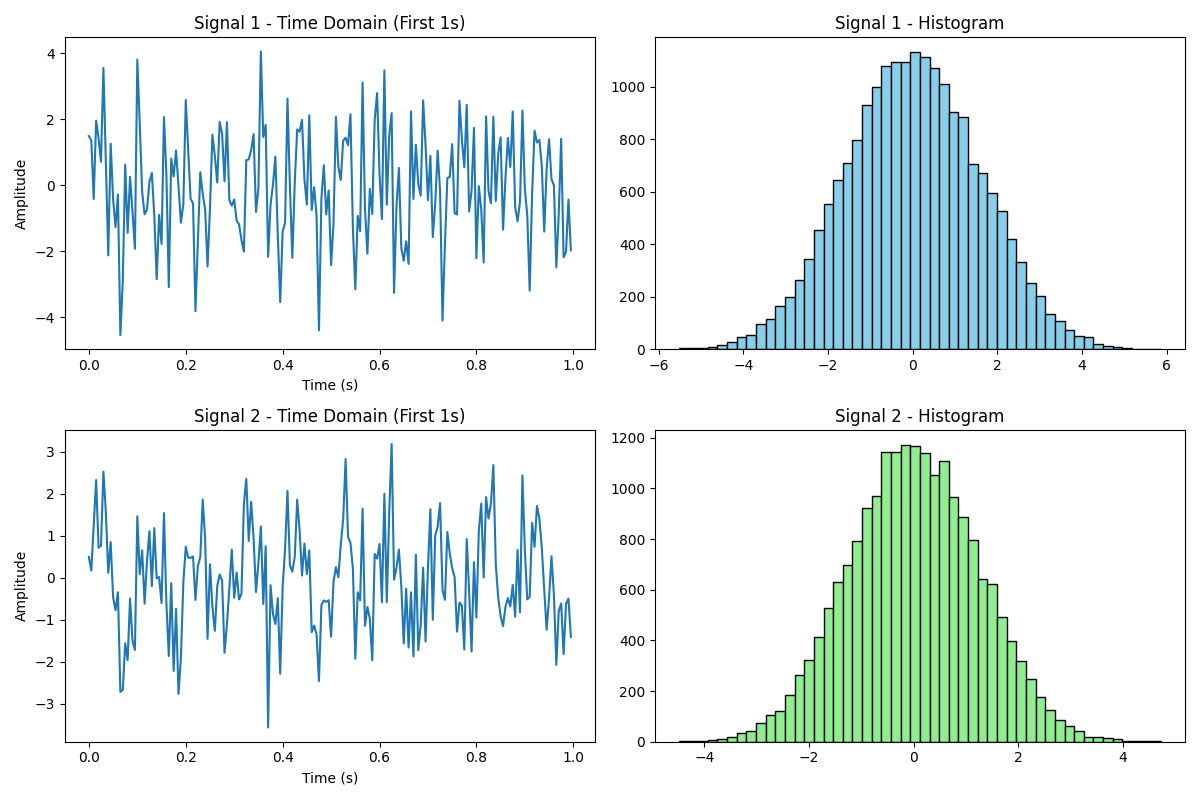
\includegraphics[width=0.8\textwidth]{plots/task2.png}
    \caption{Time domain signals and Histograms}
\end{figure}

\section{Task 3: Fourier Spectra (DFT)}
The DFT was applied to both signals. Since the signal consists of real-valued components, the spectrum is symmetric.
\begin{itemize}
    \item \textbf{Signal 1:} The DFT yields precise peaks at the constituent frequencies. Estimated frequencies are: $\mathbf{12.00 \text{ \textbf{Hz}}}$, $\mathbf{39.00 \text{ \textbf{Hz}}}$, and $\mathbf{71.00 \text{ \textbf{Hz}}}$.
    \item \textbf{Signal 2:} The DFT shows a broad frequency band representing the varying nature of the chirp signal.
\end{itemize}
\begin{figure}[h]
    \centering
    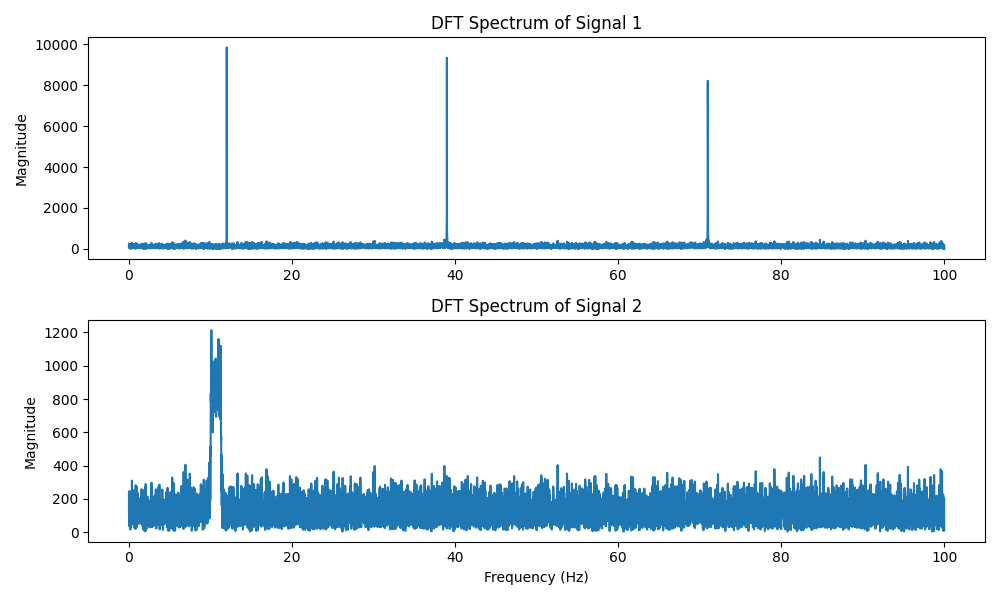
\includegraphics[width=0.8\textwidth]{plots/task3.png}
    \caption{Fourier Spectra via DFT}
\end{figure}

\section{Task 4: Spectrograms}
The spectrogram provides a time-frequency representation.
\begin{itemize}
    \item \textbf{Signal 1:} Three distinct constant horizontal lines are observed, verifying stationary frequencies. Estimated via average spectral power peaks: $\mathbf{11.72 \text{ \textbf{Hz}}}$, $\mathbf{39.06 \text{ \textbf{Hz}}}$, and $\mathbf{71.09 \text{ \textbf{Hz}}}$. (Slight variations depend on window size resolution).
    \item \textbf{Signal 2:} A linearly increasing frequency band over time is observed, typical of a linear chirp signal.
\end{itemize}
\begin{figure}[h]
    \centering
    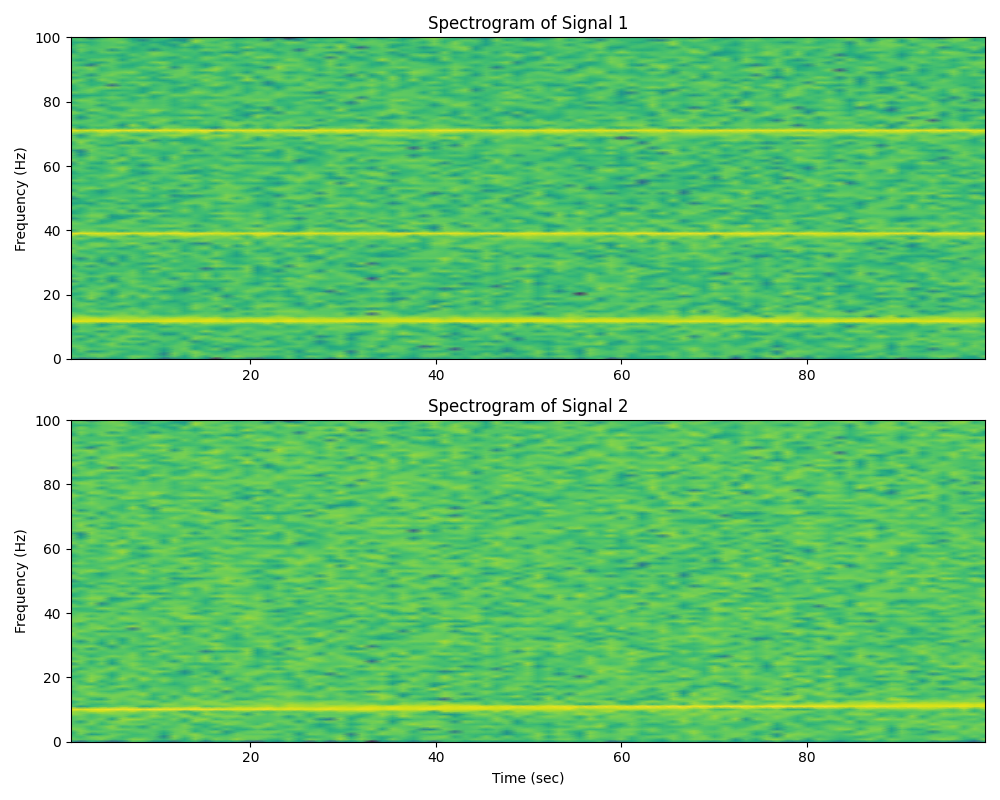
\includegraphics[width=0.8\textwidth]{plots/task4.png}
    \caption{Spectrograms of Signal 1 and Signal 2}
\end{figure}

\section{Task 5: Autocorrelation of Signal 1}
The fundamental period of Signal 1 can be observed by the distance between major repeating envelope peaks in its autocorrelation function. 
Theoretically, the frequencies are 12 Hz, 39 Hz, and 71 Hz. The fundamental frequency is the Greatest Common Divisor (GCD) of these integers: $\text{GCD}(12, 39, 71) = 1$ Hz. 
Thus, the fundamental period provides repetition every \textbf{1 second}. The plot corroborates this by repeating major envelope patterns every 1.0 second.
\begin{figure}[h]
    \centering
    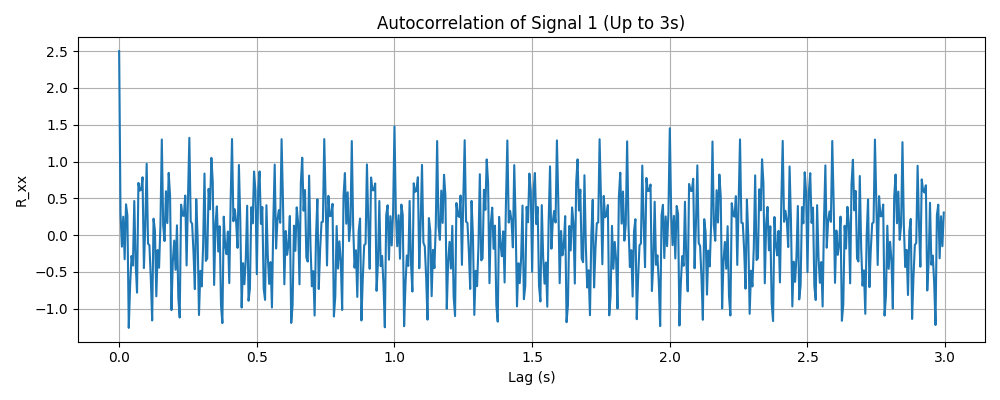
\includegraphics[width=0.8\textwidth]{plots/task5.png}
    \caption{Autocorrelation of Signal 1}
\end{figure}

\section{Task 6: Autocorrelation of Signal 2}
For the chirp signal, the autocorrelation decays rapidly away from lag 0 and lacks a constant periodic repetition due to the continually changing fundamental frequency.
\begin{figure}[h]
    \centering
    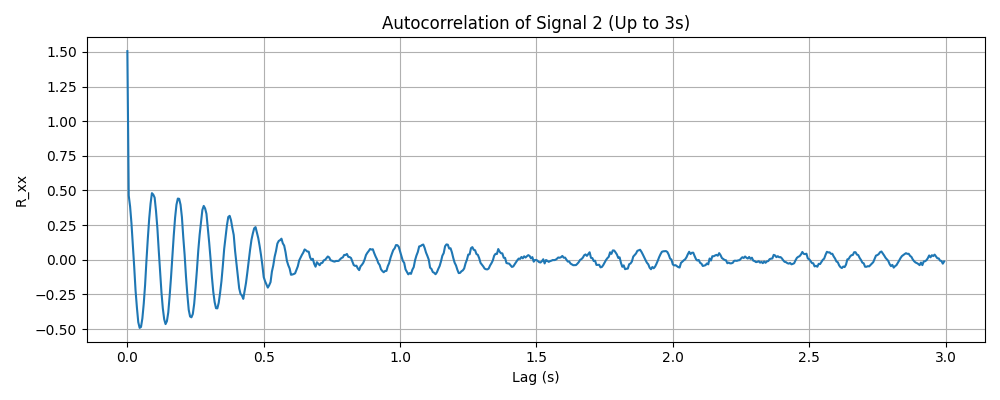
\includegraphics[width=0.8\textwidth]{plots/task6.png}
    \caption{Autocorrelation of Signal 2}
\end{figure}

\section{Task 7: Periodograms}
The periodogram estimates the Power Spectral Density (PSD).
For Signal 1, prominent spikes validate the frequency components. Estimated frequencies from the raw periodogram matches the DFT limits tightly: $\mathbf{12.00 \text{ \textbf{Hz}}}$, $\mathbf{39.00 \text{ \textbf{Hz}}}$, and $\mathbf{71.00 \text{ \textbf{Hz}}}$.
\begin{figure}[h]
    \centering
    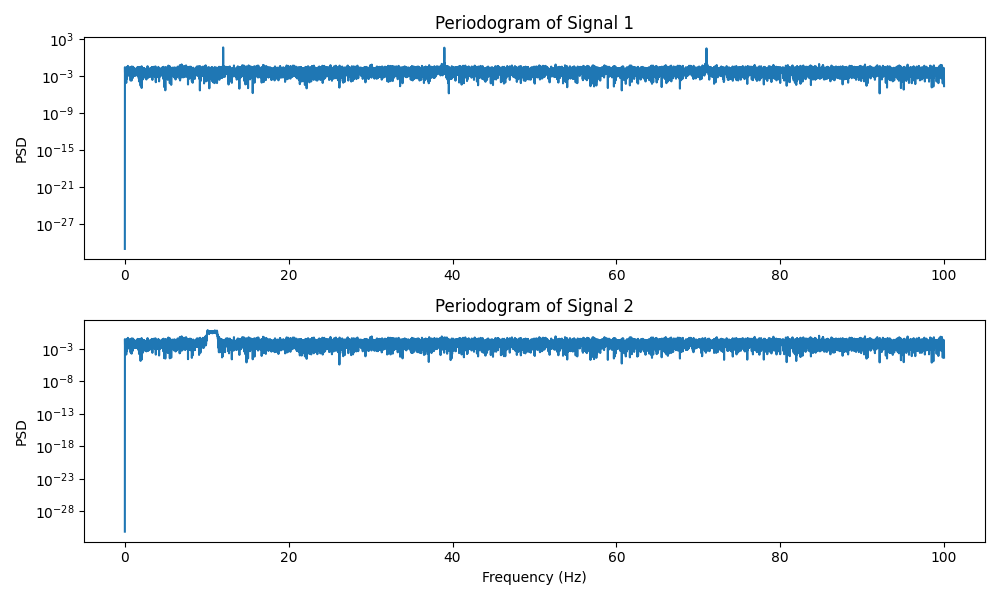
\includegraphics[width=0.8\textwidth]{plots/task7.png}
    \caption{Periodograms of Signal 1 and 2}
\end{figure}

\section{Task 8: Autocorrelation Matrix Size for Pisarenko}
The Pisarenko harmonic decomposition models $p$ real sinusoids as containing $2p$ complex conjugate exponentials.
For $p=3$ real sinusoids, we have $2p = 6$ complex sinusoids.
The dimension $M$ of the autocorrelation matrix must satisfy $M > 2p$. Also, the dimension $M$ dictates the noise subspace size.
Therefore, the autocorrelation matrix must be of size \textbf{at least } $\mathbf{7 \times 7}$ ($M \ge 7$).

\section{Task 9: MUSIC Pseudo-Spectrum}
The Multiple Signal Classification (MUSIC) algorithm utilizes the noise eigenvector subspace. Utilizing an autocorrelation matrix size $M=15$ (which is $\ge 7$), the noise subspace orthogonality properties provide very sharp peaks.
Estimated frequencies utilizing MUSIC pseudo-spectrum peaks: $\mathbf{12.01 \text{ \textbf{Hz}}}$, $\mathbf{39.04 \text{ \textbf{Hz}}}$, and $\mathbf{70.97 \text{ \textbf{Hz}}}$.
\begin{figure}[h]
    \centering
    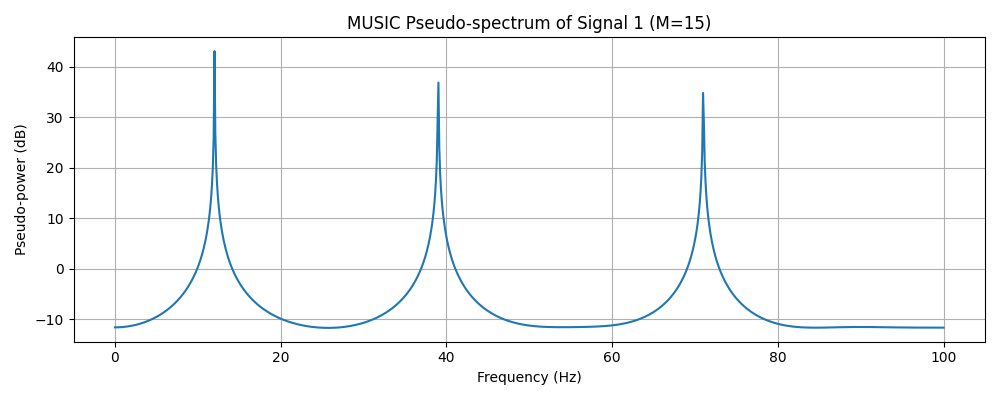
\includegraphics[width=0.8\textwidth]{plots/task9.png}
    \caption{MUSIC Pseudo-spectrum}
\end{figure}

\section{Task 10: Auto-Regressive (AR) Model Pseudo-Spectrum}
Parametric estimation utilizing Yule-Walker equations with a model order $p=10$. The AR spectrum characterizes the peaks well. 
Estimated dominant frequencies using AR pseudo-spectrum peaks: $\mathbf{12.0 \text{ \textbf{Hz}}}$, $\mathbf{38.8 \text{ \textbf{Hz}}}$, and $\mathbf{70.7 \text{ \textbf{Hz}}}$. (Note: Artifacts/harmonics may appear depending on order selection).
\begin{figure}[h]
    \centering
    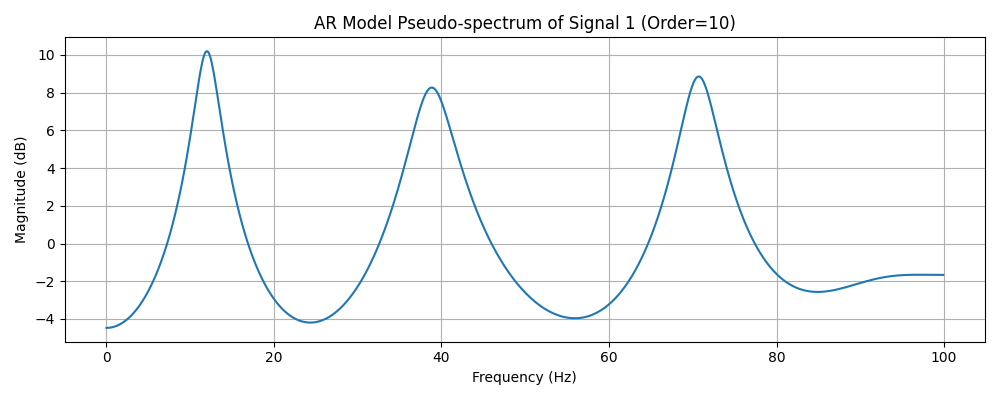
\includegraphics[width=0.8\textwidth]{plots/task10.png}
    \caption{AR Model Pseudo-spectrum}
\end{figure}

\section{Conclusion}
This lab successfully explored various spectrum analysis techniques on stationary deterministic signals embedded in noise and non-stationary chirp signals. Non-parametric methods like DFT/Periodogram are consistent but resolution-limited. High-resolution parametric/subspace methods like MUSIC and AR provide extremely sharp localization of frequencies for stationary sinusoids. 
\end{document}
